\documentclass[11pt,a4paper]{article}

\usepackage[margin=1in]{geometry}
\usepackage[T1]{fontenc}
\usepackage[utf8]{inputenc}
\usepackage{lmodern}
\usepackage{graphicx}
\usepackage{booktabs}
\usepackage{array}
\usepackage{float}
\usepackage{hyperref}
\usepackage{xcolor}
\usepackage{amsmath}
\usepackage{amssymb}
\usepackage{enumitem}
\usepackage{setspace}
\usepackage{caption}
\usepackage{tikz}
\usetikzlibrary{arrows.meta,positioning}

\hypersetup{
  colorlinks=true,
  linkcolor=blue,
  urlcolor=blue
}

\captionsetup{font=small, labelfont=bf}
\setstretch{1.08}
\setlength{\parindent}{0pt}
\setlength{\parskip}{0.72em}
\setcounter{secnumdepth}{2}
\setcounter{tocdepth}{2}

\title{Q-Learning for Mastermind:\\State History, Epsilon-Greedy Exploration, and Learning Curves}
\author{}
\date{}

\begin{document}
\maketitle
\tableofcontents
\clearpage
\phantomsection
\addcontentsline{toc}{section}{List of Figures}
\listoffigures
\clearpage
\phantomsection
\addcontentsline{toc}{section}{List of Tables}
\listoftables
\clearpage

\section*{Abstract}
\addcontentsline{toc}{section}{Abstract}

This report presents my tabular Q-learning solution for the supplied Mastermind assignment. Although the environment is small, the work involved more than filling in the update equation. The hidden code is never given to the agent, so the table has to learn from recent guess-feedback records. Because of that, I treated the task as a comparison of state memory, exploration, and training progress. One final success score would have missed too much.

The report follows the four assignment questions: implementing the update, comparing history lengths, comparing epsilon values, and plotting learning curves. The results show why the weaker settings mattered. \texttt{history\_length = 1} reaches 76.0\% mean win rate, which is above the random baseline but still not reliable. \texttt{history\_length = 2} reaches 100.0\% mean win rate and gives the best mean average-turn value among the tested history settings. For exploration, several epsilon values solve the task, but \texttt{epsilon = 0.3} gives the best tested mean average-turn value, 2.98, while keeping 100.0\% mean win rate. The learning curves then show most improvement by about 2{,}000 episodes, followed by a near-flat plateau after roughly 3{,}000 episodes.

\section{Introduction}

At first, the supplied Mastermind environment looks straightforward. Each episode asks the agent to guess a hidden code within a maximum number of turns. A guess produces feedback, and that feedback guides the next guess. Black peg feedback marks colours in the correct positions, while white peg feedback marks correct colours in incorrect positions. However, one feedback result rarely identifies the hidden code by itself. It only narrows the situation.

Using the Markov Decision Process material from \texttt{05\_mdp}, the task can be described through states, actions, rewards, and next states. The awkward part is the state. It is not the true hidden code, and it is not a full list of all possible codes left after the feedback. It is only a fixed-length history of guesses and feedback. As a result, a short history can merge different situations into the same table entry. A longer history gives more context, but it also expands the state space. Q2 is mainly about this trade-off.

Q-learning, covered in the temporal-difference material in \texttt{06\_tdlearning}, estimates values for state-action pairs and updates them after each transition. I used it because it matches the assignment structure and because it makes the difference between behaviour and learning clear. During training the agent can behave epsilon-greedily, yet the update still uses the greedy next-state value. That separation is why the method is off-policy.

The report is organised around the four assignment questions. Q1 explains the implementation. Q2 compares state-history lengths. Q3 compares epsilon values. Q4 uses learning curves to show how the selected agent improves over time. I also report the weaker or non-selected settings, because the final choices only make sense when seen against what was tried.

\section{Experimental Setup and Reproducibility}

All experiments were run from \texttt{assignment/code/student\_template.py}. I used the supplied \texttt{MastermindEnv} for the game rules and the supplied \texttt{QTable} for value storage. Their public interfaces were left unchanged, so the work stayed within the assignment structure and did not become a rewrite of the provided code.

To keep the comparisons meaningful, I held the environment settings and scaffold learning parameters fixed while varying two parameters: history length and epsilon. This mattered because changing several parts of the setup at once would make the results harder to interpret. If the win rate changed, it would no longer be clear which change caused it.

The search was therefore staged in two steps. First, I tested history length, because the state representation affects everything the Q-table can learn. Then I kept the selected history length fixed and tested epsilon. Across both sweeps, \texttt{ETA}, \texttt{GAMMA}, environment settings, run counts, training episodes, and evaluation games stayed the same.

Shared environment settings:

\begin{itemize}[leftmargin=1.5em]
  \item \texttt{NUM\_COLORS = 4}
  \item \texttt{NUM\_POSITIONS = 2}
  \item \texttt{MAX\_TURNS = 6}
  \item \texttt{ETA = 0.2}
  \item \texttt{GAMMA = 0.99}
\end{itemize}

\subsection{Controlled Assignment Settings}

History length and epsilon were the variables tested directly because they match the experimental questions in the scaffold. Other values define the supplied task, the learning rule, or the amount of evidence used for each comparison. Table~\ref{tab:fixed-settings} records those fixed settings so the results can be reproduced.

\begin{table}[H]
\centering
\caption{Controlled settings used across the experiments}
\label{tab:fixed-settings}
\small
\begin{tabular}{@{}>{\raggedright\arraybackslash}p{2.9cm} >{\raggedright\arraybackslash}p{2.5cm} >{\raggedright\arraybackslash}p{4.5cm} >{\raggedright\arraybackslash}p{4.0cm}@{}}
\toprule
Setting & Value Used & Source or Reason & Role in This Report \\
\midrule
\texttt{NUM\_POSITIONS}, \texttt{NUM\_COLORS} & 2 positions, 4 colours & Recommended assignment setting; it gives 16 possible codes/actions. & Defines the Mastermind task used for every comparison. \\
\texttt{MAX\_TURNS} & 6 & Supplied environment default. & Defines the failure cutoff and the average-turn penalty for unsolved games. \\
Reward scheme & +10 for a win, -1 otherwise & Supplied by the environment. & Gives the agent a clear terminal reward while penalising extra guesses. \\
\texttt{ETA} & 0.2 & Fixed value recommended in the scaffold for this focused study. & Controls the size of each Q-value update. \\
\texttt{GAMMA} & 0.99 & Fixed value recommended in the scaffold. & Keeps later winning rewards important over the short episode. \\
Q-table initial values & 0.0 with random greedy tie-breaking & Supplied by \texttt{QTable}. & Explains why \texttt{epsilon = 0.0} can still try different actions early on. \\
Runs and evaluation games & 10 runs, 10{,}000 training episodes, 500 final evaluation games & Chosen to report means and standard deviations across runs. & Gives each tested setting the same training and evaluation conditions. \\
\bottomrule
\end{tabular}
\end{table}

As a result, the measured comparisons focus on \texttt{history\_length} and \texttt{epsilon}. The settings in Table~\ref{tab:fixed-settings} are kept constant across those comparisons.

\subsection{How Results Were Generated}

Both \texttt{SWEEP\_RUNS} and \texttt{CURVE\_RUNS} were set to 10. This gave enough repeated runs to report means and standard deviations without making the experiment unnecessarily slow. Fixed values \texttt{ETA = 0.2} and \texttt{GAMMA = 0.99} were kept from the scaffold.

For history length, results were generated with \texttt{experiment\_history\_length(...)}. I tested histories \texttt{1, 2, 3, 4}, while epsilon was fixed at \texttt{0.2}. Each setting used 10 runs, 10{,}000 training episodes per run, and 500 evaluation games per run.

For epsilon, \texttt{experiment\_epsilon(...)} was run after history length 2 had been selected. I tested \texttt{0.0, 0.05, 0.1, 0.2, 0.3, 0.5}. The same run count and evaluation size were used again, so the epsilon comparison was not mixed with a change in evaluation method.

The learning curves used the selected pair: history length 2 and \texttt{epsilon = 0.3}. Each curve run lasted 10{,}000 training episodes, with evaluation every 500 episodes using 200 evaluation games. Failed games were counted as \texttt{max\_turns + 1} in the average-turns score, so failures still affected the score instead of disappearing from the average.

A random baseline was evaluated under the same game settings. It achieved a win rate of 30.8\% with an average-turn value of 5.92. Figures used in the report are stored in \path{assignment/results/}.

\section{Q1: Implementation}

\subsection{Understanding the Question}

Q1 first required me to make the learning step explicit. One transition changes one state-action value, so the implementation had to answer a small but important question: what should the target be after this move? Before the final guess, the answer includes a future estimate. At the final guess, it cannot.

I separated the work into two connected parts. Action selection controls how training experience is collected. The update rule then uses that experience to adjust the Q-table. If either part is wrong, the later sweeps become meaningless, because the reported history and epsilon comparisons would only be measuring a broken learner.

\subsection{Design and Settings Choices}

Action selection uses epsilon-greedy behaviour:

\begin{itemize}[leftmargin=1.5em]
  \item During training, the agent chooses a random action with probability $\epsilon$.
  \item If it does not explore, it chooses the greedy action returned by the provided Q-table.
  \item During evaluation, exploration is switched off so that the measured performance reflects the learned greedy policy.
\end{itemize}

I kept the scaffold values $\eta = 0.2$ and $\gamma = 0.99$. This kept the experiment focused on history length and epsilon. A wider hyperparameter search would have made the report less tied to the assignment questions. A high discount factor is also reasonable here because the winning reward may arrive after several guesses, not immediately after the first action.

\begin{figure}[H]
\centering
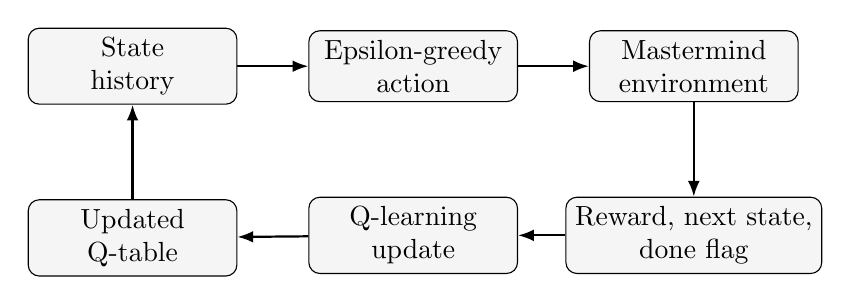
\begin{tikzpicture}[
  node distance=1.2cm and 0.9cm,
  box/.style={draw, rounded corners, align=center, minimum width=2.65cm, minimum height=0.85cm, fill=gray!8},
  arrow/.style={-{Latex[length=2mm]}, thick}
]
\node[box] (state) {State\\history};
\node[box, right=of state] (action) {Epsilon-greedy\\action};
\node[box, right=of action] (env) {Mastermind\\environment};
\node[box, below=of env] (transition) {Reward, next state,\\done flag};
\node[box, below=of action] (update) {Q-learning\\update};
\node[box, below=of state] (qtable) {Updated\\Q-table};

\draw[arrow] (state) -- (action);
\draw[arrow] (action) -- (env);
\draw[arrow] (env) -- (transition);
\draw[arrow] (transition) -- (update);
\draw[arrow] (update) -- (qtable);
\draw[arrow] (qtable) -- (state);
\end{tikzpicture}
\caption{Training-loop structure used by the tabular Q-learning agent.}
\label{fig:qlearning-loop}
\end{figure}

\subsection{Implementation}

Bellman optimality provides the basis for the update:
\[
q^*(s, a) = \mathbb{E}[r + \gamma \max_{a'} q^*(s', a') \mid s, a].
\]
This equation links the value of an action to the immediate reward and the best value available afterwards. In the tabular implementation, I used it in two cases because terminal and non-terminal transitions do not mean the same thing:

\begin{itemize}[leftmargin=1.5em]
  \item If the next state is terminal, the target is only the immediate reward.
  \item If the next state is not terminal, the target includes the discounted greedy value of the next state.
\end{itemize}

For terminal transitions:
\[
\text{target} = r.
\]
For non-terminal transitions:
\[
\text{target} = r + \gamma \max_{a'} Q(s', a').
\]

Temporal-difference error is the gap between the current table value and the target:
\[
\delta = \text{target} - Q(s, a).
\]
Finally, the Q-table is moved toward the target:
\[
Q(s, a) \leftarrow Q(s, a) + \eta \delta.
\]

\subsection{Testing, Improvement, and Final Implementation}

Terminal transitions needed careful handling. A finished game has no future action from which to bootstrap. If the update used a next-state maximum after the final step, it would add value from a decision that will never happen. Before the end of the game, however, bootstrapping is exactly the mechanism that makes TD learning useful.

Later experiments provide a basic implementation check. A broken update or action-selection rule would be expected to stay close to the random baseline of 30.8\% win rate. The trained agents move well beyond that baseline, which supports the implementation being functional.

Q-learning is off-policy in this implementation. The behaviour policy is epsilon-greedy, so it sometimes takes exploratory actions. The update target uses $\max_{a'}Q(s',a')$, which corresponds to the greedy policy. In other words, the agent learns about the greedy policy while collecting experience from a policy that sometimes explores.

\section{Q2: History Length Results}

\subsection{Understanding the Question}

Q2 asks how much previous feedback should be included in the state. I treated this as a state-design question before treating it as a score question. Too little history can make different situations look identical to the table. Too much history can increase the number of possible states without improving decisions.

The Markovian property is relevant because a useful state should contain the information needed to choose the next action. Since the assignment state is only a short memory of guesses and feedback, the experiment tests how much memory is enough for this environment. This was the first point where the task became less obvious than it first looked.

\subsection{Design and Settings}

I tested \texttt{history\_length = 1, 2, 3, 4}. This gave a small comparison from minimal memory to a longer short-term history.

\texttt{history\_length = 1} was the minimal-memory case: only the most recent guess-feedback record is stored. I used it as the baseline for the state representation, not because I expected it to be best. A length of 2 then adds one more record while still keeping the state small. Lengths 3 and 4 check whether more memory continues to improve the result, or whether it only makes the table larger.

During this sweep, epsilon was fixed at \texttt{0.2}. Each setting used 10 runs, 10{,}000 training episodes per run, and 500 evaluation games per run. Keeping epsilon fixed was important because this experiment was meant to isolate the effect of state history.

\subsection{Measured Results}

Table~\ref{tab:history} gives the measured win rates and average-turn values for every tested history length. Figure~\ref{fig:history} shows the same comparison as a plot, with the random baseline included as a reference point. I included all tested settings here because the selected value only makes sense when the weaker and non-selected values are visible as well.

\begin{table}[H]
\centering
\caption{History-length sweep results for all tested settings}
\label{tab:history}
\begin{tabular}{>{\ttfamily}c c c}
\toprule
History Length & Win Rate & Average Turns \\
\midrule
1 & 76.0\% $\pm$ 10.6\% & 4.11 $\pm$ 0.31 \\
2 & 100.0\% $\pm$ 0.0\% & 2.95 $\pm$ 0.12 \\
3 & 100.0\% $\pm$ 0.0\% & 3.01 $\pm$ 0.09 \\
4 & 100.0\% $\pm$ 0.0\% & 3.01 $\pm$ 0.20 \\
\bottomrule
\end{tabular}
\end{table}

\begin{figure}[H]
\centering
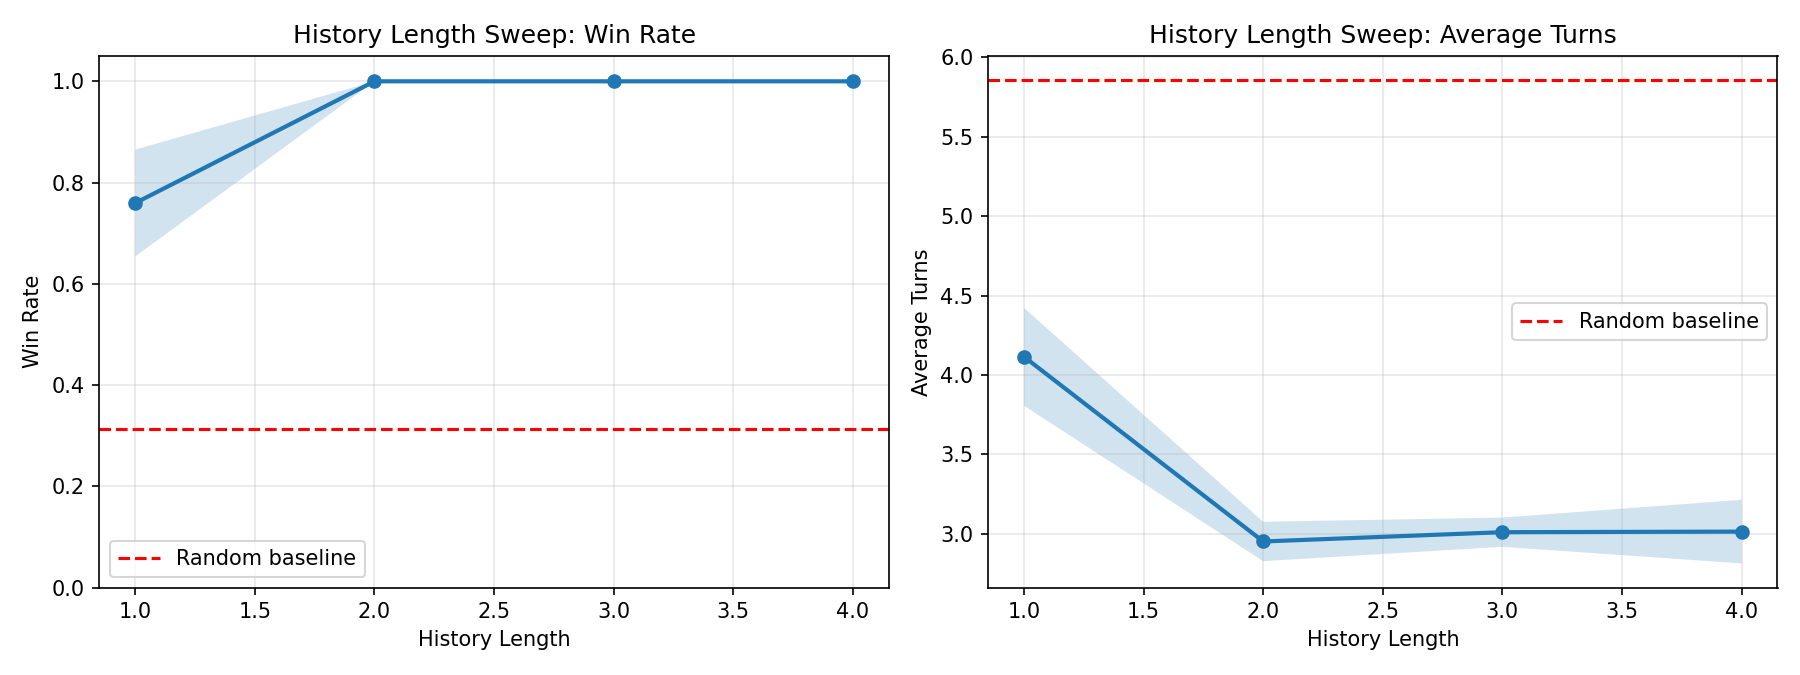
\includegraphics[width=\textwidth]{results/history_length_comparison.png}
\caption{History-length comparison for all tried settings, showing win rate and average turns with variability bands and the random baseline.}
\label{fig:history}
\end{figure}

\subsection{Testing, Interpretation, and Refinement}

\texttt{history\_length = 1} was not a complete failure. It reached 76.0\% mean win rate, which is clearly above the random baseline. However, it was not reliable, and the standard deviation of 10.6\% shows that performance still varied across runs. One guess-feedback record gives useful information, but not enough for steady play.

\texttt{history\_length = 2} changed the result sharply. It reached 100.0\% mean win rate and gave the best average-turn value in the history sweep, at 2.95. That extra stored feedback appears to separate situations that were ambiguous with only one previous record.

\texttt{history\_length = 3} and \texttt{history\_length = 4} also solved the task, reaching 100.0\% mean win rate. Despite this, neither improved the mean average-turn value. They also increase the state space beyond what was needed. In hindsight, these two settings were still useful to test because they showed where the benefit of extra memory stopped.

\subsection{Final Decision}

\begin{table}[H]
\centering
\caption{History-length selection summary}
\label{tab:history-summary}
\small
\begin{tabular}{@{}>{\raggedright\arraybackslash}p{1.2cm} >{\raggedright\arraybackslash}p{3.2cm} >{\raggedright\arraybackslash}p{4.5cm} >{\raggedright\arraybackslash}p{3.7cm}@{}}
\toprule
Setting & Why Tried & What Happened & Decision \\
\midrule
1 & Minimal-memory case; tests whether one feedback record is enough & Learns above random baseline, but only reaches 76.0\% mean win rate and has weaker turns & Rejected because runs are not steady enough \\
2 & First state augmentation beyond the minimal case & Jumps to 100.0\% mean win rate and gives the best mean turns, 2.95 & Selected as the smallest successful history \\
3 & Checks whether extra memory improves on length 2 & Also reaches 100.0\%, but mean turns are slightly worse at 3.01 & Not selected; no measured gain \\
4 & Checks whether still longer short-term history helps & Also reaches 100.0\%, but mean turns remain 3.01 and state size is larger & Not selected; extra state growth without benefit \\
\bottomrule
\end{tabular}
\end{table}

For Q2, the final choice is \texttt{history\_length = 2}. It gives enough state information without adding more states than the agent needs.

\section{Q3: Exploration Results}

\subsection{Understanding the Question}

Q3 asks how much exploration should be used during training. Epsilon controls how often the agent ignores the current greedy action and samples a random action. At first, it is tempting to assume that more exploration will always help. The results make that too simple. Exploration can help the agent find useful actions, but too much random action selection can make training less steady.

\subsection{Design and Settings}

After selecting \texttt{history\_length = 2}, I tested \texttt{epsilon = 0.0, 0.05, 0.1, 0.2, 0.3, 0.5}. The sweep moves from no epsilon-forced random actions to a high-exploration case.

\texttt{epsilon = 0.0} tests whether learning still occurs without epsilon-driven random actions. \texttt{0.05} and \texttt{0.1} test low exploration. \texttt{0.2} and \texttt{0.3} test moderate exploration. \texttt{0.5} gives a high-exploration comparison, where random actions are more likely to interrupt the greedy behaviour being learned.

Each setting used 10 runs, 10{,}000 training episodes per run, and 500 evaluation games per run. The chosen history length was kept fixed throughout this sweep.

\subsection{Measured Results}

Table~\ref{tab:epsilon} reports the measured results for the full epsilon sweep, including the values that were not selected. Figure~\ref{fig:epsilon} gives the same comparison as a plot.

\begin{table}[H]
\centering
\caption{Epsilon sweep results for \texttt{history\_length = 2} across all tested settings}
\label{tab:epsilon}
\begin{tabular}{>{\ttfamily}c c c}
\toprule
Epsilon & Win Rate & Average Turns \\
\midrule
0.0 & 100.0\% $\pm$ 0.0\% & 3.08 $\pm$ 0.21 \\
0.05 & 100.0\% $\pm$ 0.0\% & 3.16 $\pm$ 0.26 \\
0.1 & 100.0\% $\pm$ 0.0\% & 3.08 $\pm$ 0.17 \\
0.2 & 100.0\% $\pm$ 0.0\% & 3.05 $\pm$ 0.13 \\
0.3 & 100.0\% $\pm$ 0.0\% & 2.98 $\pm$ 0.15 \\
0.5 & 99.4\% $\pm$ 1.7\% & 3.07 $\pm$ 0.19 \\
\bottomrule
\end{tabular}
\end{table}

\begin{figure}[H]
\centering
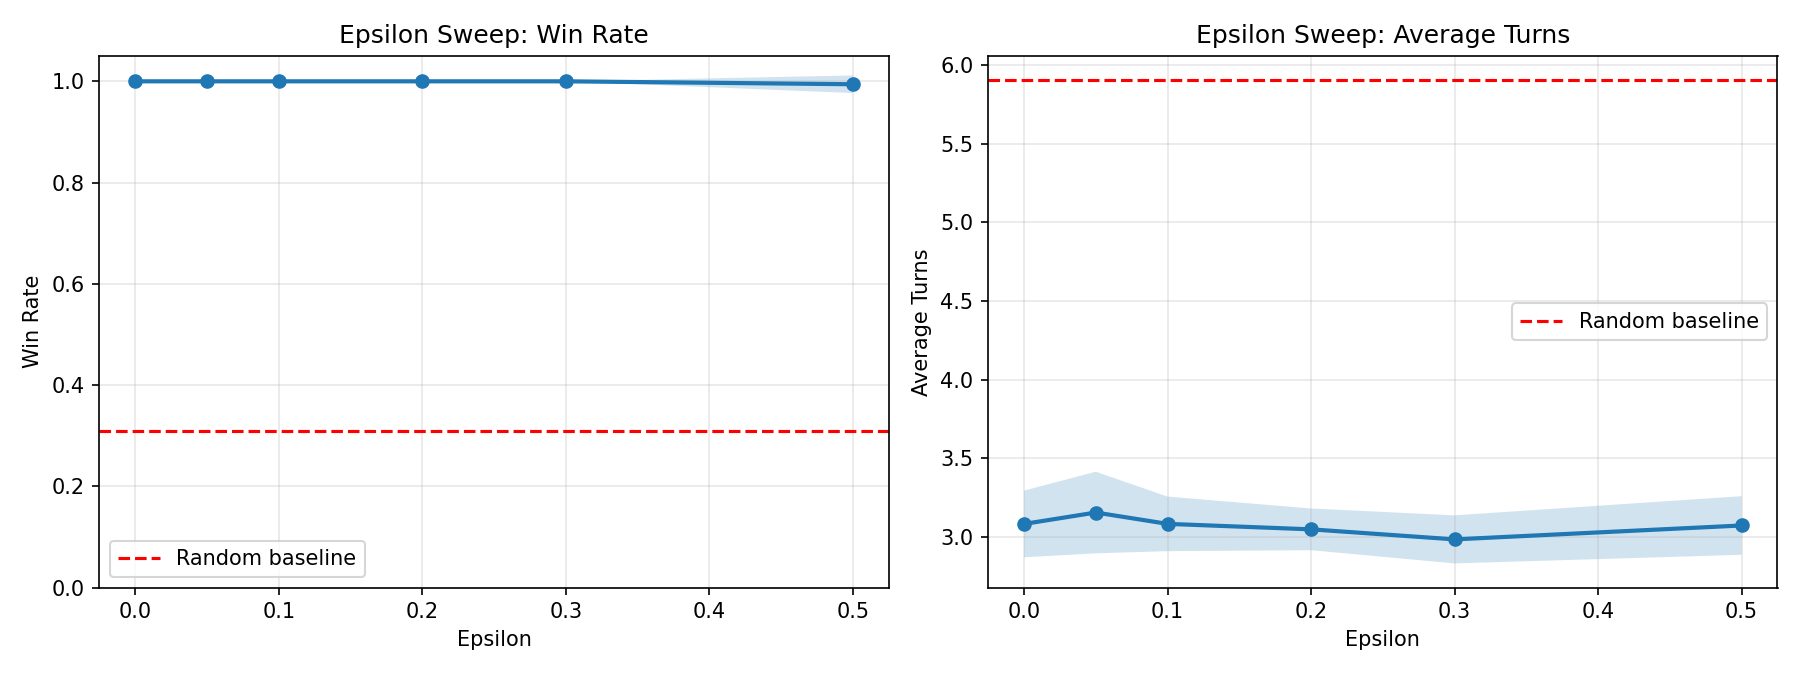
\includegraphics[width=\textwidth]{results/epsilon_comparison.png}
\caption{Epsilon comparison for all tried settings, showing win rate and average turns with variability bands and the random baseline.}
\label{fig:epsilon}
\end{figure}

\subsection{Testing, Interpretation, and Refinement}

\texttt{epsilon = 0.0} still reached 100.0\% mean win rate, even though epsilon itself never forces a random action. This does not mean exploration is irrelevant. The supplied Q-table provides another early source of random choice: unseen Q-values start equal, and \texttt{QTable.get\_best\_action} breaks ties randomly. With a small action space, that tie-breaking was enough to support learning.

\texttt{epsilon = 0.05} and \texttt{epsilon = 0.1} were also reliable, both reaching 100.0\% mean win rate. Their average-turn scores were not better than the moderate settings, especially \texttt{0.05}, which had the weakest mean turns among the perfect-win-rate epsilon values at 3.16.

\texttt{epsilon = 0.2} was close. It reached 100.0\% mean win rate with mean turns of 3.05. \texttt{epsilon = 0.3} also reached 100.0\% mean win rate and had the lowest mean average-turn value, 2.98. The gap is small, so the conclusion should stay modest: moderate exploration worked well here, and \texttt{0.3} was the best measured value in this sweep.

\texttt{epsilon = 0.5} became the first clearly weaker exploration setting. It was the only tested value with a mean win rate below 100.0\%, and it did not improve average turns. At this level, random actions began to reduce the win rate.

\subsection{Final Decision}

\begin{table}[H]
\centering
\caption{Epsilon selection summary}
\label{tab:epsilon-summary}
\small
\begin{tabular}{@{}>{\raggedright\arraybackslash}p{1.45cm} >{\raggedright\arraybackslash}p{3.05cm} >{\raggedright\arraybackslash}p{4.55cm} >{\raggedright\arraybackslash}p{3.45cm}@{}}
\toprule
Setting & Why Tried & What Happened & Decision \\
\midrule
0.0 & Edge case with no epsilon-forced exploration & Still reaches 100.0\% mean win rate because random tie-breaking gives early random actions & Strong, but not the best turn score \\
0.05 / 0.1 & Low explicit exploration & Both reach 100.0\%, but mean turns are 3.16 and 3.08 & Reliable, but less efficient than the selected setting \\
0.2 & Moderate exploration & Reaches 100.0\% with mean turns of 3.05 & Close result, but slightly weaker than 0.3 on mean turns \\
0.3 & Moderate exploration & Reaches 100.0\% and gives the best mean turns, 2.98 & Selected as the best tested epsilon \\
0.5 & High-exploration case & Drops to 99.4\% mean win rate and gives no turn-score advantage & Rejected as the first clear win-rate drop \\
\bottomrule
\end{tabular}
\end{table}

For Q3, the final choice is \texttt{epsilon = 0.3}. Evaluation is then run with \texttt{explore=False}, because the purpose is to evaluate the learned greedy policy without training-time random actions mixed into the score.

\section{Q4: Learning Dynamics}

\subsection{Understanding the Question}

Q4 asks what happens during training as well as what happens at the end. A final score can hide whether the agent learned quickly, learned slowly, or only succeeded in a lucky run. The learning curve is needed because it shows the process, not just the final state of the process.

\subsection{Design and Settings}

For the final experiment, I used the selected settings from Q2 and Q3: history length 2 with \texttt{epsilon = 0.3}. It used 10 independent runs, 10{,}000 training episodes, and evaluation every 500 episodes using 200 games. The shaded bands show standard deviation across runs.

\subsection{Measured Learning Path}

Figure~\ref{fig:curves} shows the mean learning curves and standard-deviation bands.

\begin{figure}[H]
\centering
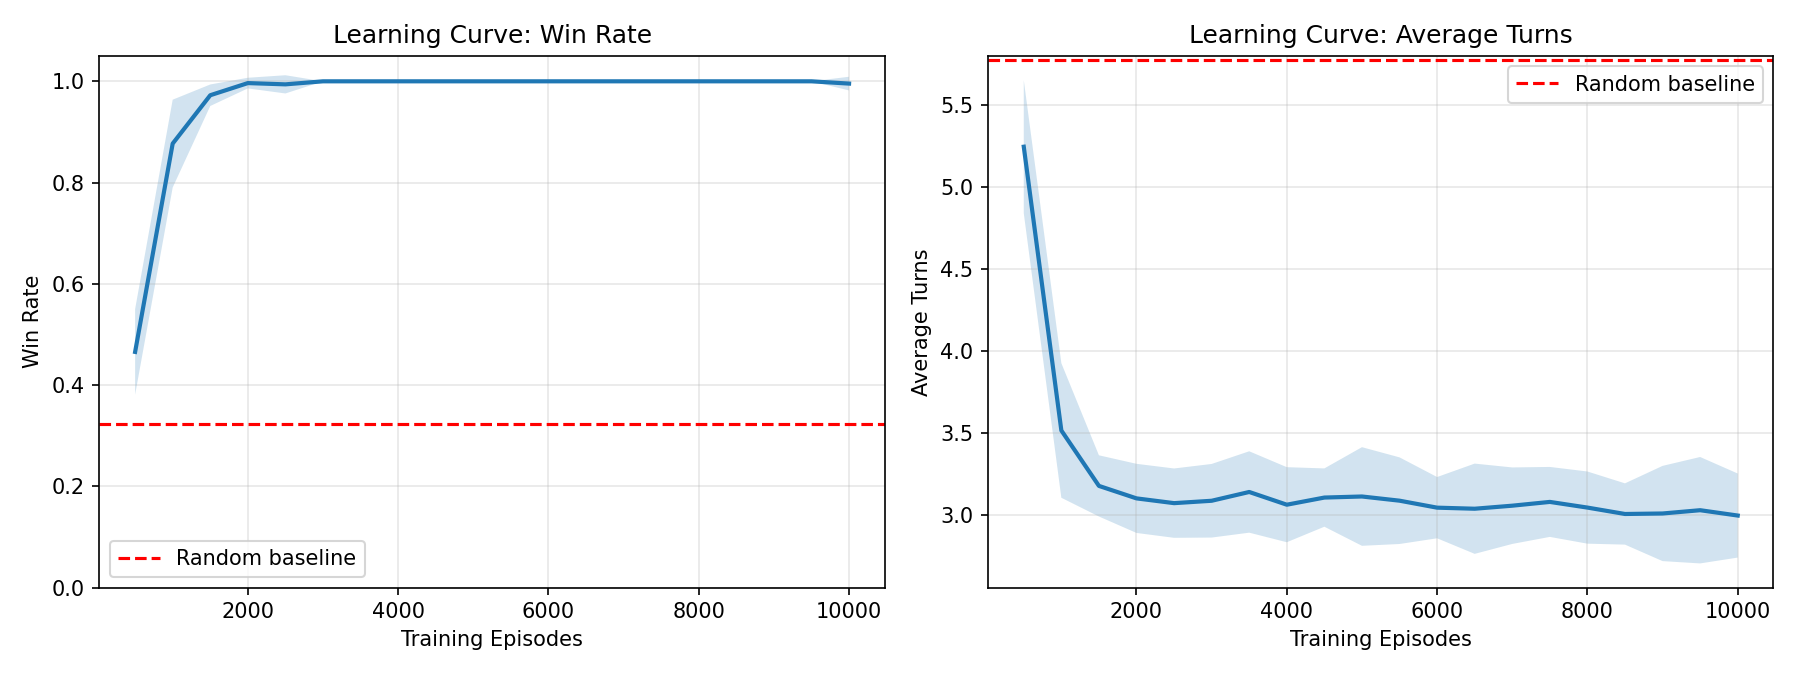
\includegraphics[width=\textwidth]{results/learning_curves.png}
\caption{Learning curves for the final chosen setting, with mean and standard-deviation bands over multiple runs.}
\label{fig:curves}
\end{figure}

A three-stage reading makes the learning curve clearer:

\begin{itemize}[leftmargin=1.5em]
  \item Early training is still unstable. At 500 episodes, the mean win rate is 46.6\%, and the mean average-turn score is 5.244.
  \item The next 1{,}500 episodes produce most of the improvement. By 1{,}000 episodes, the mean win rate is 87.7\%; by 1{,}500 episodes, it is 97.2\%; and by 2{,}000 episodes, it reaches 99.6\%.
  \item After about 3{,}000 episodes, the win-rate curve is almost flat at 100.0\%. The average-turn score stays close to 3.0 and ends at 2.998 after 10{,}000 episodes.
\end{itemize}

Training beyond the flat part of the curve is still useful as a check across runs. It does not change the conclusion about the selected setting, but it makes the result harder to dismiss as an early lucky plateau.

\begin{table}[H]
\centering
\caption{Learning-curve milestones for the final chosen setting}
\label{tab:milestones}
\begin{tabular}{>{\ttfamily}c c c}
\toprule
Episodes & Mean Win Rate & Mean Average Turns \\
\midrule
500 & 46.6\% & 5.244 \\
1{,}000 & 87.7\% & 3.516 \\
1{,}500 & 97.2\% & 3.179 \\
2{,}000 & 99.6\% & 3.103 \\
3{,}000 & 100.0\% & 3.089 \\
10{,}000 & 100.0\% & 2.998 \\
\bottomrule
\end{tabular}
\end{table}

\subsection{Testing, Run Variation, and Average Turns}

Multiple runs are needed because TD algorithms are stochastic, as discussed in the course material. The agent's experience depends on random exploratory actions, random greedy tie-breaking, and the sequence of hidden codes during training. One run can look unusually good or poor, so means and standard deviations give a better summary.

Average turns are measured more strictly than an average over successful games only. Failed games are counted as \texttt{max\_turns + 1}. As a result, the score penalises both slow solutions and failures. Without that convention, a weak agent could look artificially efficient by averaging only the few games it happened to solve.

\subsection{Final Interpretation}

By roughly 2{,}000 episodes, the final setting reaches high win rate; by around 3{,}000 episodes, the curve is almost flat. After that point, extra training mainly checks that the result is steady across repeated runs.

\section{Conclusion}

This implementation uses tabular Q-learning with epsilon-greedy training behaviour and a greedy evaluation policy. Its update separates terminal and non-terminal transitions, and uses the greedy next-state value in the non-terminal target. That matches the off-policy Q-learning method covered in the temporal-difference learning material.

The results support \texttt{history\_length = 2} as the final state-history setting. A history length of one gives the agent some useful information, but not enough for reliable play. Lengths three and four work, but they do not improve the measured result and make the state space larger than necessary.

For exploration, \texttt{epsilon = 0.3} is the selected training value. This is not because all other values fail. Several values work, and zero epsilon works because of random greedy tie-breaking in the supplied Q-table. The reason for selecting \texttt{0.3} is narrower: among the tested values, it gives the best mean average-turn result while keeping 100.0\% mean win rate.

Recommended final setting:

\begin{itemize}[leftmargin=1.5em]
  \item \texttt{history\_length = 2}
  \item \texttt{epsilon = 0.3}
\end{itemize}

With these settings, the agent reaches 100.0\% final mean win rate in the reported experiments. Most of the useful policy is learned within the first few thousand episodes, and the state history is not larger than it needs to be. Overall, the assignment changed from a simple implementation task into a question of evidence: what information the agent needed, how much exploration was useful, and when the learning curve had stopped changing in a meaningful way.

\end{document}
